\section{Façade}

Quando um subsistema possui muitas interfaces 
de acesso às suas funcionalidades, o acesso de 
classes clientes de outros subsistemas a ele 
torna-se descentralizado, aumentando a dependência 
entre os dois sistemas. Para minimizar esse problema, 
o padrão Façade fornece uma interface generalizada 
para todo o subsistema, de forma que as classes 
clientes possam comunicar-se apenas com um ponto 
de entrada. A figura \ref{facade_struct} demonstra 
o padrão, onde uma classe Façade, que é o ponto de 
acesso ao subsistema, possui uma referência para 
os componentes que antes eram diretamente acessíveis.

\begin{figure}[htb]
	\caption{\label{facade_struct}Estrutura do Façade}
	\begin{center}
	    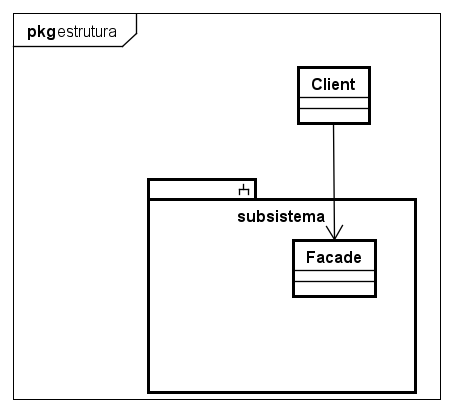
\includegraphics[scale=0.4]{5_padroes-contexto-funcional/5.2_estruturais/5.2.5_facade/facade_estrutura.png}
	\end{center}
\end{figure}

\subsection*{Exemplo Orientado a Objetos}

Como exemplo de uso do Façade, pode-se considerar 
um compilador que oferece diversas funcionalidades. 
Essas funcionalidades são apresentadas no diagrama 
de classes da figura \ref{facade_exemplo}, representadas 
pelas classes Scanner, Parser, ProgramNodeBuilder e 
CodeGenerator. Por mais que alguns clientes desejem 
acessar essas funcionalidades diretamente, a maioria 
deseja apenas compilar seu programa, sem importar-se 
com as etapas necessárias para isso. Assim, ao invés de 
criar uma dependência entre o cliente e as 
funcionalidades, a classe Compiler fornece um ponto 
de acesso a todas elas, permitindo que um cliente 
que deseja apenas compilar seu código possa fazer 
isso diretamente. O código \ref{oofacade} demonstra 
a implementação desse exemplo.

\begin{figure}[htb]
	\caption{\label{facade_exemplo}Exemplo de Façade}
	\begin{center}
	    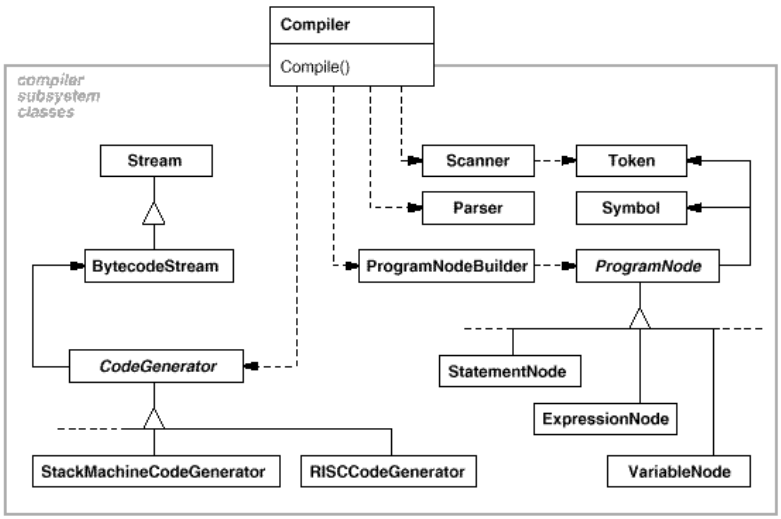
\includegraphics[scale=0.4]{5_padroes-contexto-funcional/5.2_estruturais/5.2.5_facade/facade_exemplo.png}
	\end{center}
\end{figure}


\begin{lstlisting}[caption={Façade Orientado a Objetos},label=oofacade]

class Scanner(val input : Stream[String]) {
  def Scan() : Token = {
    //Recupera token na stream de código fonte
  }
}

class Parser {
  def Parse(scanner : Scanner, builder : ProgramNodeBuilder) : SyntacticTree[ProgramNode] = {
    //Retorna a árvore de análise
  }
}

class ProgramNodeBuilder(var rootNode : ProgramNode) {
  // Possui os métodos para criação dos nós do programa
}

class CodeGenerator() {
  // Possui os métodos para gerar o código de máquina do programa
  def Traverse(rootNode : ProgramNode) : Stream[Byte] = {
    // Percorre a árvore e gera o bytecode
  }
}

class Compiler {
  def Compile(input : Stream[String]) : Stream[Byte] = {
    val scanner = new Scanner(input)
    val programNodeBuilder = new ProgramNodeBuilder(null)
    val parser = new Parser();

    parser.Parse(scanner, programNodeBuilder);

    val codeGenerator = new CodeGenerator();
    val parseTree = programNodeBuilder.rootNode;

    codeGenerator.Traverse(parseTree);
  }
}

\end{lstlisting}

\subsection*{Contexto Funcional}

Esse padrão pode ser implementado de duas formas: 
definindo um módulo que é utilizado como ponto de 
acesso para outros módulos ou definindo uma 
função dentro de um módulo que é um ponto de 
acesso para outras funções não exportadas do 
mesmo módulo. Independente da forma utilizada, 
a função Compile, que é o ponto de acesso, permanece 
a mesma. Ela pode ser vista no código \ref{facadecompile}. 

Para que essa função seja implementada de forma 
funcional, a implementação vista no código \ref{oofacade} 
foi alterada para que seja utilizada uma composição 
de funções. Na linha 5, a função Scan é chamada, 
seu resultado é passado para a função Parse, cujo 
resultado é passado para a função Traverse. Essa sim, 
retorna a \textit{stream} de \textit{bytes} com o 
código compilado do programa.

\begin{lstlisting}[caption={Função de acesso Compile},label=facadecompile]
    
object Compiler {

  def Compile(input: Stream[String]): Stream[Byte] = {
    (Traverse compose Parse compose Scan) (input)
  }
  
}
    
\end{lstlisting}

O código \ref{facademodules} demonstra o primeiro caso, 
onde as operações utilizadas pela função Compile são 
definidas em módulos separados. Apenas o módulo 
Compiler precisa conhecer e importar essas funções.

\begin{lstlisting}[caption={Função de acesso Compile},label=facademodules]
    
object Scanner{
  private def Scan(input : Stream[String]) : Scanner = 
    // Faz o scan do código fonte
}

object Parser{
  private def Parse(scanner : Scanner)
  : ProgramNodeBuilder = 
    // Gera a árvore abstrata sintática com os tokens
}

object CodeGenerator{
  private def Traverse(builder : ProgramNodeBuilder) : Stream[Byte] = 
    // Percorre a árvore para gerar o código de máquina
}

\end{lstlisting}

Para o segundo exemplo, o código \ref{facadepvtfunc} define 
as funções como membros não exportados do módulo Compiler. 
Dessa forma, o módulo cliente não conseguirá acessá-los, 
precisando acessar suas funcionalidades apenas através da 
função Compile.

\begin{lstlisting}[caption={Função de acesso Compile},label=facadepvtfunc]
    
  // módulo Compiler    

  private def Scan(input : Stream[String]) : Scanner = 
    // Faz o scan do código fonte

  private def Parse(scanner : Scanner)
  : ProgramNodeBuilder = 
    // Gera a árvore abstrata sintática com os tokens

  private def Traverse(builder : ProgramNodeBuilder) : Stream[Byte] = 
    // Percorre a árvore para gerar o código de máquina
    
\end{lstlisting}

\subsection*{Vantagens e Desvantanges}

A implementação funcional desse padrão não apresenta 
vantagens ou desvantagens, tendo em vista que ela apenas 
depende da forma como a linguagem separa ou agrupa 
suas implementações - seja através de classes ou módulos. 